\documentclass[tikz,border=2pt]{standalone}
\usepackage{pgfplots}
\usepgfplotslibrary{polar,ternary}
\pgfplotsset{compat=1.18}
\begin{document}
\begin{tikzpicture}
\begin{axis}[
  x filter/.code={\ifdim\thisrow{x}pt<1pt\def\pgfmathresult{}\fi}
]
\addplot table {
x y
0 0
1 1
2 4
3 9
};
\end{axis}
\end{tikzpicture}

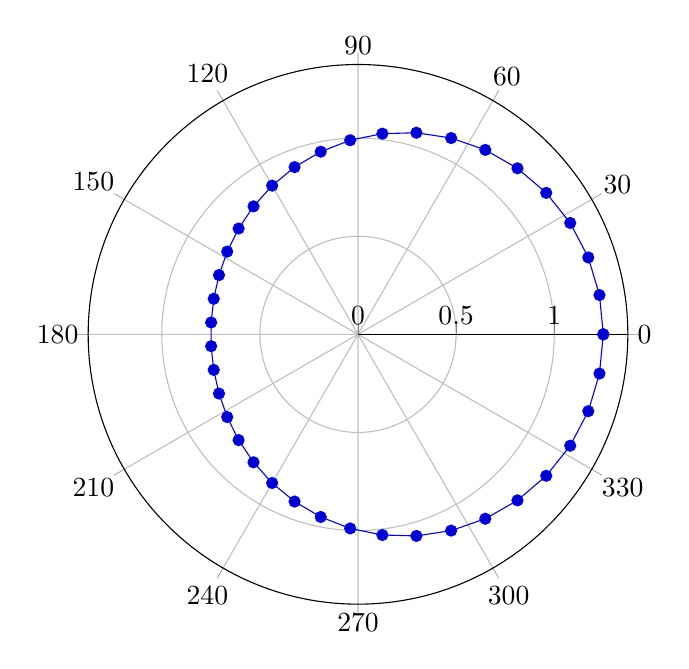
\begin{tikzpicture}
\begin{polaraxis}
\addplot+[domain=0:360,samples=40] {1+0.25*cos(x)};
\end{polaraxis}
\end{tikzpicture}

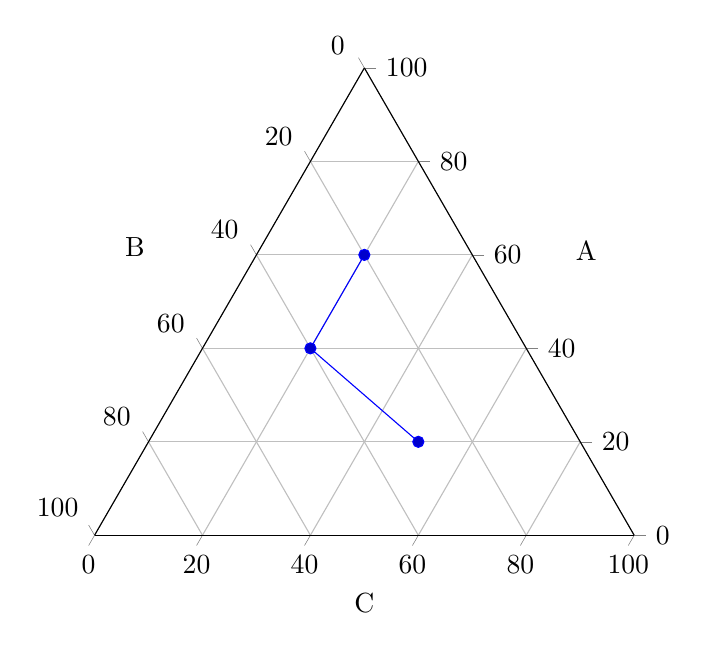
\begin{tikzpicture}
\begin{ternaryaxis}[xlabel={A},ylabel={B},zlabel={C}]
\addplot3 coordinates {
  (0.2,0.3,0.5)
  (0.4,0.4,0.2)
  (0.6,0.2,0.2)
};
\end{ternaryaxis}
\end{tikzpicture}
\end{document}
